\section{Circuito n° 2}

\subsection{Análisis Teórico}

Se realiza el análisis teórico del circuito que se muestra en la siguiente figura. 


\begin{figure}[H]
    \centering
    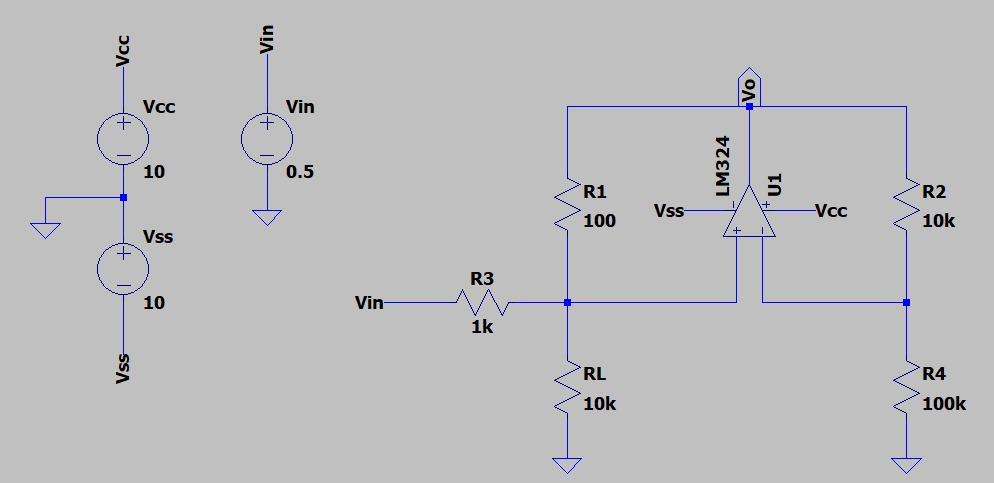
\includegraphics[width=0.7\linewidth]{Circuito2.jpg}
    \caption{Circuito n° 2}
\end{figure}

Inicialmente expresamos v+ y v- en función de Vo planteando el divisor resistivo en el nodo ‘2’ de la figura:

\[v^+ = v^- = V_0  \frac{R_4}{R_4 + R_2} \]

\[\frac{V_{in}}{R_3} + \frac{V_o}{R_1} = v^+ (\frac{1}{R_L}+\frac{1}{R_1}+\frac{1}{R_3}) \]

Reemplazando v+:

\[\frac{V_{in}}{R_3} + \frac{V_o}{R_1} = V_0  \frac{R_4}{R_4 + R_2} (\frac{1}{R_L}+\frac{1}{R_1}+\frac{1}{R_3})\]

\[{V_{in}} = V_0  R_3 [ \frac{R_4}{R_4 + R_2} (\frac{1}{R_L}+\frac{1}{R_1}+\frac{1}{R_3})\]

\[{V_{in}} = V_0 \left[ \frac{1}{R_L}(R_3 \frac{R_4}{R_4 + R_2}) + R_3\frac{R_4}{R_4 + R_2}(\frac{1}{R_1}+\frac{1}{R_3})-\frac{R_3}{R_1} \right] \]

Reemplazando para $ R1 = 100\,\Omega, R2 = 10\,k\Omega, R3 = 1\,k\Omega, R4 = 100\,k\Omega $ :

% \[{V_{in}} = V_0 \left[ \frac{909,09091}{R_L} \right]\]
\[{V_{in}} = V_0 \left[ \frac{10000}{11\,R_L} \right]\]

Ahora, vamos a expresar la corriente que fluye a través de la carga en
función del valor de la carga resistiva y de la tensión de entrada :


\[I_{RL}= \frac{v^+}{R_L}\]
\[I_{RL}= V_o\frac{R_4}{R_4 + R_2} \frac{1}{R_L}\]


\[I_{RL}=\frac{V_{in}}{\left[\frac{1}{R_L}(R_3{R_4}{R_4 + R_2})\right]}\frac{R_4}{R_4 + R_2}\frac{1}{R_L}\]

\[I_{RL}= \frac{V_{in}}{R_3}\]

\[I_{RL}= V_{in}.10^{-3}\]

También podemos expresar la amplitud de la tensión de salida en función de la tensión de entrada y de la carga:

\[V_{out} = \frac{V_{in}}{\frac{1}{R_L}909.09091}\]

\[V_{out} = V_{in}R_L*1.1*10^-3\]

Para terminar, podemos encontrar la relación entre el valor máximo de la carga que podemos conectar al circuito y la tensión de entrada. Para determinar la RL máxima, debemos considerar el caso en el cual Vo sea igual a Vcc (10V):

\[10[V] = V_{in}R_L*1.1*10^-3\]
\[R_{L,mac} = \frac{909.09091}{V_{in}}\]


A partir de la relaciones que pudimos encontrar analíticamente, completamos las tablas de las figuras \ref{fig:IRL_vs_carga} y \ref{fig:Vo_vs_carga}. En estas tablas, se pueden encontrar valores de la corriente a través de la carga y respectivamente de la tensión de salida para Vin=[0.5;1;2]V y RL= [0,1,2,5,10]k.

\begin{figure}[H]
    \centering
    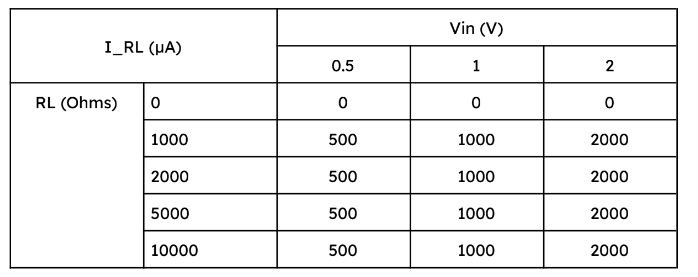
\includegraphics[width=0.7\linewidth]{Secciones/Circuito2/Tabla3.png}
    \caption{Valor teórico de la amplitud de la corriente en la carga en función del valor de la carga y de la amplitud de la tensión de entrada}
    \label{fig:IRL_vs_carga}
\end{figure}

\begin{figure}[H]
    \centering
    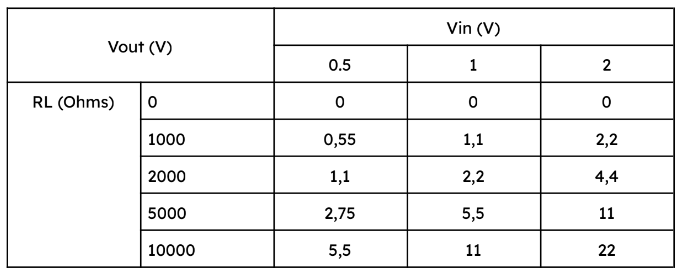
\includegraphics[width=0.7\linewidth]{Secciones/Circuito2/Tabla4.png}
    \caption{Valor teórico de la amplitud de la tensión de salida en función del valor de la carga y de la amplitud de la tensión de entrada}
    \label{fig:Vo_vs_carga}
\end{figure}

Cabe aclarar que aquellos valores de tensión de salida que superen Vcc (10V) implican que la señal estará recortada.


\subsection{Simulacion}
Después de hacer el análisis teórico del circuito, lo simulamos utilizando LTSpice. En el osciloscopio de simulación, medimos la amplitud de la corriente de la carga para distintos valores de la misma y varios valores de tensión de entrada. Los resultados son presentados en la siguiente tabla.

\begin{table}[h!]
\centering
\begin{tabular}{|c|c|c|c|}
\hline
\textbf{RL [ohm]} & \textbf{I [A] (0.5 V)} & \textbf{I [A] (1 V)} & \textbf{I [A] (2 V)} \\ \hline
1K    & 498.78 $\mu$  & 999.16 $\mu$  & 2 m \\ \hline
2K    & 496.9 $\mu$  & 996.2 $\mu$  & 2 m \\ \hline
5K    & 495.98 $\mu$  & 994 $\mu$  & 1.55 m \\ \hline
10K   & 493.9 $\mu$  & 771.1 $\mu$  & 783.2 $\mu$ \\ \hline
\end{tabular}
\caption{Corriente según la carga RL.}
\label{tab:iL_vs_RL}
\end{table}
Luego, realizando un barrido de $V_{in}$ variando ademas la carga, obtenemos las siguientes gráficas.

\begin{figure}[H]
    \centering
    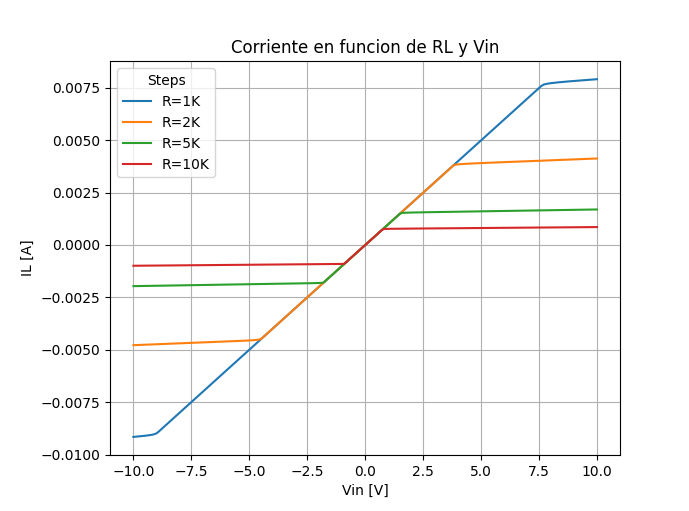
\includegraphics[width=0.70\linewidth]{Secciones/Circuito2/TP1_2_i_vs_Vin_RL.png}
    \caption{Simulacion de la corriente por la carga}
\end{figure}

Para el analisis de la tension de salida Vo con diferentes valores de carga y tension de entrada Vin:

\begin{table}[h!]
\centering
\begin{tabular}{|c|c|c|c|}
\hline
\textbf{RL [ohm]} & \textbf{Vo [V] (0.5 V)} & \textbf{Vo [V] (1 V)} & \textbf{Vo [V] (2 V)} \\ \hline
1K    & 0.546  & 1.096  & 2.19  \\ \hline
2K    & 1.092  & 2.19   & 4.38  \\ \hline
5K    & 2.72   & 5.46   & 8.47  \\ \hline
10K   & 5.43   & 8.45   & 8.5  \\ \hline
\end{tabular}
\caption{Tensión de salida según la carga RL.}
\label{tab:Vo_vs_RL}
\end{table}
\begin{figure}[h!]
    \centering
    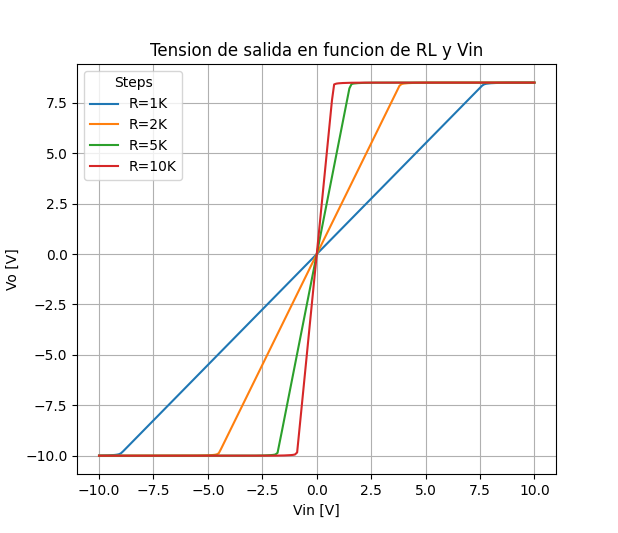
\includegraphics[width=0.70\linewidth]{Secciones/Circuito2/TP1_2_Vo_vs_Vin_RL.png}
    \caption{Simulacion de la corriente por la carga}
\end{figure}


%\subsection{II.4. Comparación de los resultados teóricos, de simulación y calculados}

%A continuación se muestra una tabla comparativa de los resultados obtenidos tanto en simulación como experimentalmente y los calculados para una resistencia
%RL de $1k\Omega$ (ver Figura 23). También, calculamos los errores relativos entre los
%resultados obtenidos experimentalmente, por simulación y por análisis teórico.
%Viendo los errores relativos de la Figura 23, notamos que como para el
%estudio del primer circuito el error relativo entre simulación y teoría es el más pequeño. También podemos observar que los errores relativos experimento/teórico y experimento/simulación son por lo menos dos veces más pequeños que para el circuito 1 (con un error máximo de 10.7 %).
%Esto podría ser debido a que en el circuito 2, solamente utilizamos un amplificador operacional en vez de 2.



